% !TEX TS-program = pdflatexmk
% !BIB TS-program = bibtex

\documentclass[12pt, a4paper, oneside]{book}
\usepackage{import}
\subimport{../}{preamble}
\ExecuteBibliographyOptions{articletitle=false}
\standalonetrue
\onehalfspacing
\begin{document}

\begin{singlespace}
{\color{white}
\chapter{Theoretical Background and Literature}}
\label{ch:theory}
\end{singlespace}

\AddToShipoutPictureBG*{ \AtPageUpperLeft{ \put(0,-240)
{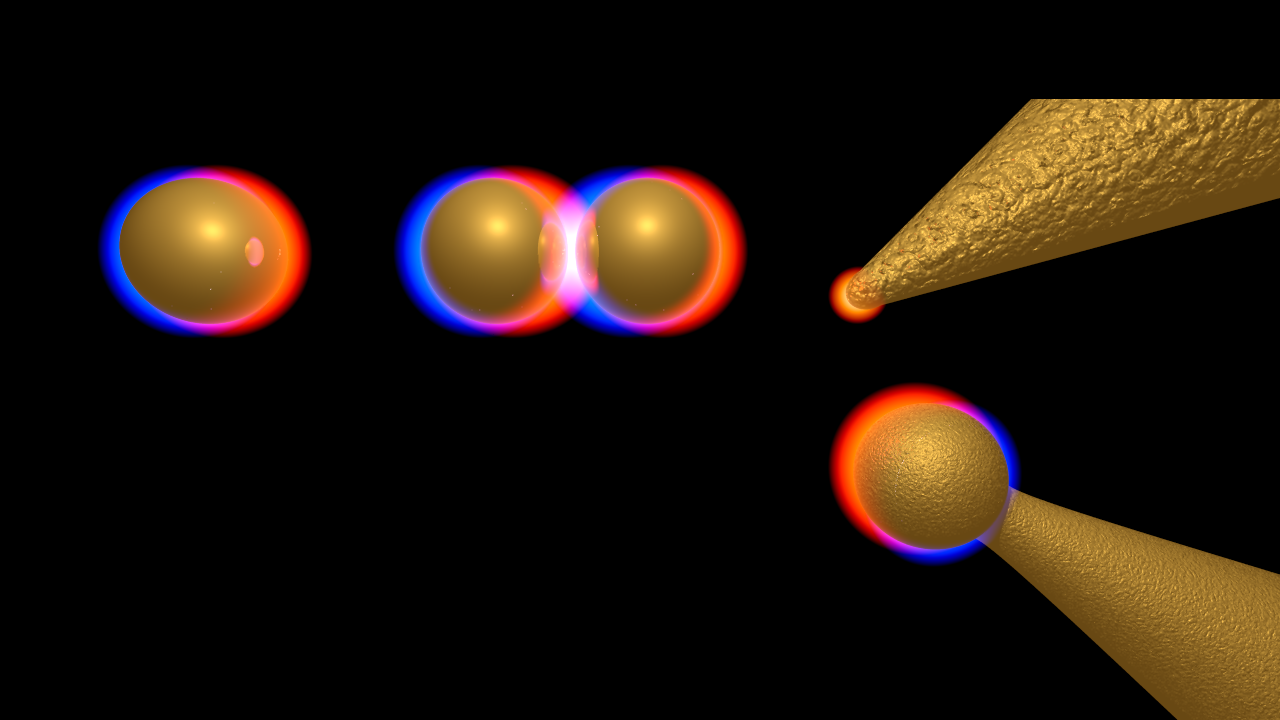
\includegraphics[width=\paperwidth, clip=true, trim=0 100 0 100]{data/chapter_cover.png}}
}}

This ability to confine light below the diffraction limit can be achieved by exploiting plasmons. By transferring energy from a diffraction-limited photonic field into resonantly polarised, collective oscillations of conduction electrons an enhanced electric field can be generated on the surface of a metallic nanostructure with nanoscale localisation. It is through the understanding and application of this phenomena that sub-wavelength optics is made possible.
This chapter deals firstly with electromagnetic waves in media and the optical properties of metals. From this basis the existence of plasmons can be explained, including the different types of plasmons and how they interact within different spatial regimes. Through this, the study of charge transfer in plasmonic systems in motivated. Finally, the plasmonics of metallic tips is discussed as these are the structures primarily dealt with in this project to study plasmon interaction through each of the characteristic spatial regimes.

\subimport{./}{plasmons}
\subimport{./}{plasmon_coupling}

% How is the tip experiment different to static systems
Although charge transfer effects have been shown in previous reports by varying the conductivity of a fixed gap, there has yet to be a report showing the optical response of a dynamic dimer structure correlated with its electronic response. It is the aim of this project to successfully demonstrate and explain the possible ways in which electrical and optical plasmonic phenomena {\color{red}intertwine/become entangled} using a dual plasmonic nano-tip dimer. So far plasmons in planar and {\color{red}spherical/spheroidal} geometries have been discussed, however many other geometries of metallic nanostructure support plasmons. Tips are one such geometry, currently receiving significant attention, that have been shown to support both \glspl{spp} and \glspl{lsp}. In order to use nano-tips in determining the effects of quantum tunnelling on plasmonics, their supported plasmons must first be understood.

\subimport{./}{tip_plasmonics_literature}

\section{Conclusions}

Charge transfer effects in plasmonic systems are a phenomenon still requiring significant investigation. The influence of electron tunnelling has only been touched upon in recent years. Tips, if possessing far-field antenna plasmons, provide a useful platform for studying fundamental plasmonics in a dynamic way. Their well-developed experimental geometries for topological measurements form the basis of microscopes integrating optics and tips. By using such a setup, the quantum regime of tunnelling plasmonics can be further investigated.

To date there has been no direct correlated measurements between plasmon resonances and quantum tunnelling. Tunnelling has been inferred from direct measurements of plasmon resonances without electronic measurements \cite{savage2012, scholl2013} and from variables influenced by the gap field enhancement, though in some cases with electronic measurements \cite{tan2014, zhu2014, hajisalem2014, cha2014}. The effects of tunnelling, specifically the relations between screening and \gls{ctp} excitation, can be better understood with correlated electrical and force measurements. By using an experimental geometry related to AFM these measurements become possible.

\ifstandalone
\begin{singlespace}
\fontsize{8pt}{1em}\selectfont
\printbibliography[notcategory=fullcited]
\end{singlespace}
\fi

\end{document}